\documentclass[11pt]{article}
\usepackage[utf8]{inputenc}
\usepackage[T1]{fontenc}
\usepackage[francais]{babel}
\usepackage[francais]{layout}
\usepackage{bm}
\selectlanguage{french}

% NE PAS CHANGER !!
\ifx \public \undefined \def\public{etudiants} \fi
\usepackage[\public]{tps}

% Numéro du TP
\newcommand{\numtd}{04}
% Titre du TP
\newcommand{\titretd}{Entiers et virgule flottante}

\def\bool{\mathrm{I\!B}}
\def\tup#1{\langle{#1}\rangle}

\graphicspath{{imgs/}}

\begin{document}

\entete{\numtd}{\titretd}

\begin{introduction}
Ce TP est consacré à des exercices sur les entiers et les nombres à virgule
flottantes.
\end{introduction}

% {{{ Opérations binaires

\section{Opérations binaires}

Le langage C dispose de mécanismes de manipulation de bits. Par exemple,
considérons deux variables $x$ et $y$ de type entier et l'opérateur $\oplus$
(xor). Notons respectivement $x_i$ et $y_i$ le $i^{ieme}$ bit de $x$ et de $y$.
Le résultat de $x \oplus y$ est le mot $z$ tel que $z_i = x_i \oplus y_i$.

Les opérateurs C sont \verb+&+ (et), \verb+|+ (ou), \verb+^+ (xor) et \verb+~+ (not). 

\noindent \textbf{Attention:} ne pas confondre les opérateurs logiques tel que
\verb+&&+, \verb+||+, etc, avec les opérateurs de manipulation
des mots binaires. En effet, là où \verb+4&2+ vaut 0, \verb+4&&2+ vaut 1.

Les opérations binaires peuvent être condensées. Ainsi \verb+x=x|2+
peut s'écrire \verb+x|=2+, et \verb+x=x^y+ peut se noter \verb+x^=y+.
Le langage fournit également les opérateurs de décalage à droite \verb+>>+
ou à gauche \verb+<<+.

\begin{enumerate}
 \item Que fait le code suivant :

\begin{verbatim}
 n & (n-1)
\end{verbatim}

% {{{ Solution
\begin{solution}
Supprime le 1 de poids le plus faible (si $n\ne0$). Vaut 0 si $n=0$.
\end{solution}
\begin{remarque}
En laisser les étudiants déduire un test pour vérifier si $n$ est puissance de 2.
\end{remarque}
% }}}

 \item Dans le code suivant $c$ et $n$ sont des entiers :
\begin{verbatim}
for (c = 0; n != 0; n &= (n-1)) c++;
\end{verbatim}
 Quelle valeur prend $c$ en fonction des valeurs de $n$ ?

% {{{ Solution
\begin{solution}

Exemple avec $n=5$.

$c=0$ ; $n\ne0$ donc \verb+n&(n-1)+ soit \verb+5&4+, en binaire \verb+101&100+,
donc $n=(100)_2$ et $c=1$

$n$ est supérieur à 0 donc \verb+4&3+ soit \verb+100&011+
donc $n=0$ et $c=2$

$c$ est le nombre de 1 dans la représentation binaire de $n$.
\end{solution}
\begin{remarque}
Voir \verb+compter1.c+.
\end{remarque}
% }}}

\item On va étudier une méthode qui compte efficacement le nombre de 1
 dans un mot de longueur $2^k$ (pour un $k\ge0$), c'est à dire dans
 $\mathcal{O}(k)$ opérations, en supposant que $2^k$ est la taille d'un
 registre.

 Soit $l\le k$ et $n$ un mot de longueur $2^k$.
 On appelle \emph{$l$-bloc} les blocs de $2^l$ bits consécutifs dans $n$
 tel que ces blocs ne se chevauchent pas. (Par exemple, il y a huit 2-blocs
 de longueur 4~dans un mot de 32~bits.) Le \emph{$l$-compte} de $n$
 est le mot de longueur $2^k$ tel que
 chacun de ses $l$-blocs contient le nombre de 1 du
 $l$-bloc correspondant dans $n$.
 Trivialement, tout mot égale son propre $0$-compte.
 On cherche à produire le $k$-compte de $n$.
 
\begin{remarque}
Par exemple, le 1-compte de $00\ 01\ 10\ 11$ est le mot $00\ 01\ 01\ 10$.
\end{remarque}

Dans ce qui suit, on va supposer que $k=5$, et du coup on travaille
avec les registres de 32 bits. La méthode est pourtant facile à généraliser.

\begin{enumerate}
\item Trouvez une opération qui produit le 1-compte de $n$
 (en temps constant).
\begin{solution}
 Dans une copie de \verb-n-, on garde les bits sur les positions paires,
 dans une autre les positions impaires. En décalant l'une des copies,
 on peut faire l'addition de tous les blocs en même temps.

 \verb-((n & 0xaaaaaaaa) >> 1) + (n & 0x55555555)-

 On remarque que les additions sont indépendantes car tout bloc est
 suffisamment grand pour stocker le nombre de 1 du mot d'origine.
\end{solution}

\item Généraliser et itérer cette opération pour calculer
 le $5$-compte de $n$.
\begin{solution}
On génère progressivement le 1-compte, puis le 2-compte etc.

 \verb-n = ((n & 0xaaaaaaaa) >> 1) + (n & 0x55555555);-\\
 \verb-n = ((n & 0xcccccccc) >> 2) + (n & 0x33333333);-\\
 \verb-n = ((n & 0xf0f0f0f0) >> 4) + (n & 0x0f0f0f0f);-\\
 \verb-n = ((n & 0xff00ff00) >> 8) + (n & 0x00ff00ff);-\\
 \verb-n = ((n & 0xffff0000) >> 16) + (n & 0x0000ffff);-
\end{solution}

\begin{remarque}
Voir \verb+compter2.c+.
\end{remarque}

\end{enumerate}

\item On travaille avec des registres de 64 bits. Soit $n=(stuvwxyz)_2$
 un octet, avec $s$ le bit le plus significatif et $z$ le moins significatif.
 Que donne l'expression C suivante ?

\begin{verbatim}
(n * 0x0202020202 & 0x010884422010) % 1023
\end{verbatim}

\begin{remarque}
On peut laisser les étudiants jouer avec \verb+bits.c+ pour qu'ils se
fassent une idée, et ensuite discuter les opérations une par une.
\end{remarque}

\begin{solution}
Cette expression invertit l'ordre des bits, elle donne $(zyxwvuts)_2$.
Par exemple, si $n=(00101101)_2=45$, l'expression donne $(10110100)_2=180$.

Explications :

Une multiplication avec \verb+0x0101010101+ donnerait simplement cinq copies
de $n$, soit :
$$(stuvwxyz\ stuvwxyz\ stuvwxyz\ stuvwxyz\ stuvwxyz)_2$$
Du coup, la multiplication avec \verb+0x0202020202+ obtient le même résultat,
mais décalé par une position à gauche. De ce fait, tout bit sur une position
paire dans $n$ se déplace vers une position impaire (et vice versa).
Si en plus on regarde des blocs de 10 bits (au lieu de 8), on obtient :
$$(s\ tuvwxyzstu\ vwxyzstuvw\ xyzstuvwxy\ zstuvwxyz0)_2$$

On marquera par-dessous chaque bit les informations suivantes :
(i) la position $i$ du bit dans $n$ (avec $0\le i\le 7$) ;
(ii) $7-i$; (iii) la position du bit dans son bloc de 10.
Par ailleurs, on marquera en gras chaque position où (ii) égale (iii).
$$
\setlength\tabcolsep{1pt}
\begin{tabular}{ccccccccccccccccccccccccccccccccccccccccccccc}
$\bm{s}$&\ \ &$t$&$u$&$v$&$w$&$\bm{x}$&$y$&$z$&$s$&$\bm{t}$&$u$&\ \ &$v$&$w$&$x$&$\bm{y}$&$z$&$s$&$t$&$\bm{u}$&$v$&$w$&\ \ &$x$&$y$&$\bm{z}$&$s$&$t$&$u$&$\bm{v}$&$w$&$x$&$y$&\ \ &$z$&$s$&$t$&$u$&$v$&$\bm{w}$&$x$&$y$&$z$&0\\
\textbf{7}&\ \ &6&5&4&3&\textbf{2}&1&0&7&\textbf{6}&5&\ \ &4&3&2&\textbf{1}&0&7&6&\textbf{5}&4&3&\ \ &2&1&\textbf{0}&7&6&5&\textbf{4}&3&2&1&\ \ &0&7&6&5&4&\textbf{3}&2&1&0&-\\
\textbf{0}&\ \ &1&2&3&4&\textbf{5}&6&7&0&\textbf{1}&2&\ \ &3&4&5&\textbf{6}&7&0&1&\textbf{2}&3&4&\ \ &5&6&\textbf{7}&0&1&2&\textbf{3}&4&5&6&\ \ &7&0&1&2&3&\textbf{4}&5&6&7&-\\
\textbf{0}&\ \ &9&8&7&6&\textbf{5}&4&3&2&\textbf{1}&0&\ \ &9&8&7&\textbf{6}&5&4&3&\textbf{2}&1&0&\ \ &9&8&\textbf{7}&6&5&4&\textbf{3}&2&1&0&\ \ &9&8&7&6&5&\textbf{4}&3&2&1&-\\[10pt]
\hline\\
\textbf{1}&\ \ &0&0&0&0&\textbf{1}&0&0&0&\textbf{1}&0&\ \ &0&0&0&\textbf{1}&0&0&0&\textbf{1}&0&0&\ \ &0&0&\textbf{1}&0&0&0&\textbf{1}&0&0&0&\ \ &0&0&0&0&0&\textbf{1}&0&0&0&0\\
1 & \ \ & \multicolumn{4}{c}{0} & \multicolumn{4}{c}{8} & \multicolumn{5}{c}{8} & \multicolumn{4}{c}{4} & \multicolumn{4}{c}{4} & \ \ & \multicolumn{4}{c}{2} & \multicolumn{4}{c}{2} & \multicolumn{5}{c}{0} & \multicolumn{4}{c}{1} & \multicolumn{4}{c}{0}\\[10pt]
\hline\\
$s$&\ \ &0&0&0&0&$x$&0&0&0&$t$&0&\ \ &0&0&0&$y$&0&0&0&$u$&0&0&\ \ &0&0&$z$&0&0&0&$v$&0&0&0&\ \ &0&0&0&0&0&$w$&0&0&0&0\\

\end{tabular}
$$

Par-dessous la première ligne, on note (en binaire ex hexadécimal) le mot
qui masque toutes les positions où (ii) égale (iii). Le <<et>> logique entre
$n$ et ce mot donne le résultat par-dessous la deuxième ligne que l'on
appelle $m$.

Chaque bit de $n$ apparaît une seule fois dans $m$, et dans
la bonne position pour l'inversion, modulo 10. Le résultat final
peut donc être obtenu en prenant le <<ou>> logique entre les cinq blocs
-- ou bien, étant donné que les bits non-zéro ne se chevauchent point,
par l'addition de ces blocs.

Notons $N:=2^{10}-1=1023$, alors
$m=\sum_{i=0}^4 k_i\cdot(N+1)^i$ pour des facteurs $k_0,\ldots,k_4\le255<N$.
Le modulo étant distributif par rapport à l'addition et la multiplication,
on obtient
$$k_i\cdot(N+1)^i=k_i\cdot1^i=k_i\pmod N$$
et du coup $m=\sum_{i=0}^4k_i\pmod N$.
\end{solution}

\end{enumerate}

% }}}

% {{{ Séquence de De Bruijn

\section{Trouver le bit de poids le plus faible}

\begin{remarque}
Mentionner qu'il existe une méthode triviale
(décaler $x$ à droite et compter jusqu'à ce que $x\&1$ donne 1),
mais cette méthode est de temps $\mathcal{O}(n)$ pour les mots
de longueur $n$. Ou bien, on se crée un tableau qui contient la
solution pour chacun des $2^n$ mots possibles, ce qui rend possible
un lookup en temps constant ($\mathcal{O}(1)$), mais avec un très grand tableau.
Notre méthode prend $\mathcal{O}(1)$ temps et nécessite un tableau
de taille $\mathcal{O}(n)$.
\end{remarque}

Dans cette partie nous étudierons une méthode pour efficacement trouver
la position du bit de 1 du poids le plus faible dans un mot binaire.
Soit $x\ne0$ un entier, du coup sa représentation contient au moins un bit de 1.
Par exemple, si la représentation binaire de $x$ est $10011000$, alors le bit
recherché est le 1 suivi par les trois zéros finaux. Dans ce
cas, on note $\ell(x)=3$. L'objectif est de trouver $\ell(x)$ pour un $x\ne0$
donné. On présente cette méthode pour les mots de $2^3=8$ bits, mais elle
peut être généralisée à $2^n$ bits pour n'importe quelle valeur de $n>0$.

La première étape consiste à étudier les séquences dites de \emph{De Bruijn}.
Soit $\bool:=\{0,1\}$ et $\bool^n$ l'ensemble des mots binaires de longueur $n$.
Une séquence de De Bruijn d'ordre $n$ est un mot binaire qui contient
tout élément de $\bool^n$.

\begin{enumerate}
\item 
 Donnez une borne inférieure triviale pour la longueur d'une séquence
 de De Bruijn d'ordre $n$.

\begin{solution}
Il y a $2^n$ mots différents dans $\bool^n$.
Une borne inférieure triviale pour une séquence $s$ est donc
de $2^n+(n-1)$, étant donné que chaque mot dans $\bool^n$
doit commencer à une position différente de $s$ et doit être suivi
par $n-1$ bits de plus.
\end{solution}
\end{enumerate}

Le graphe $G_n$ (\emph{graphe de De Bruijn d'ordre $n$})
permet de construire des séquences d'ordre $n$.
Les sommets de $G_n$ sont les éléments de $\bool^n$.
Les sommets $b_1b_2...b_n$ et $c_1c_2...c_n$ sont liés par des
arrêtes orientées si et seulement si $b_2=c_1,b_3=c_2,...b_n=c_{n-1}$.
Autrement dit, un sommet est lié au suivant en
supprimant son premier bit et en ajoutant un des bits possibles à la fin.
La Figure~\ref{DeBruijnOrdre2} représente $G_2$.

\begin{figure}[h]
 \centering
 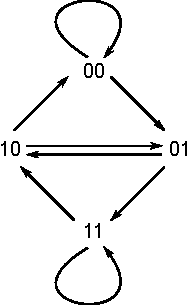
\includegraphics{order-2}
 \caption{\label{DeBruijnOrdre2}Le graphe $G_2$.}
\end{figure}


\begin{enumerate}
\setcounter{enumi}{1}
\item Dessinez le graphe $G_3$.

% {{{ Solution

\begin{solution}
\centerline{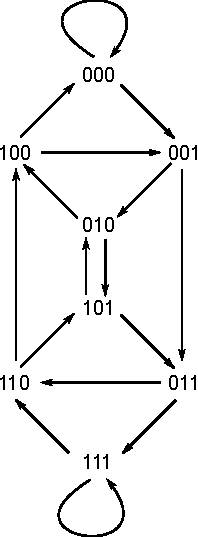
\includegraphics{order-3}}
\end{solution}
\end{enumerate}

% }}}

Une séquence de De Bruijn d'ordre $n$ correspond à un cycle hamiltonien dans
$G_n$. Un cycle hamiltonien est un cycle passant uniquement une fois par
tous les sommets du graphe avant de revenir au point de départ.
On va considérer des cycles commençant et se terminant par le sommet 000.
Par exemple, le seul cycle hamiltonien de
la figure~\ref{DeBruijnOrdre2} page~\pageref{DeBruijnOrdre2} est 00
$\rightarrow$ 01 $\rightarrow$ 11 $\rightarrow$ 10 $\rightarrow$ 00.
Pour obtenir une séquence De Bruijn, il convient de commencer par noter
le sommet initial (00) et les bits rajoutés à la fin de chaque sommet,
ce qui donne, dans ce cas, 00110. On peut prouver qu'il existe un cycle
hamiltonien dans chaque graphe de De Bruijn (voir Annexe).

\begin{enumerate}
\setcounter{enumi}{2}
\item Trouvez deux séquences de De Bruijn d'ordre 3 en utilisant
le graphe $G_3$ dessiné précédemment.  

% {{{ Solution

\begin{solution}

000 $\rightarrow$ 001 $\rightarrow$ 010 $\rightarrow$ 101 $\rightarrow$ 011
$\rightarrow$ 111 $\rightarrow$ 110 $\rightarrow$ 100

0001011100

000 $\rightarrow$ 001 $\rightarrow$ 011 $\rightarrow$ 111 $\rightarrow$ 110
$\rightarrow$ 101 $\rightarrow$ 010 $\rightarrow$ 100

0001110100

\end{solution}
\end{enumerate}

% }}}

Choisissez une séquence de De Bruijn d'ordre 3 que l'on va appeller $s$
par la suite. Si $s$ est composée de bits $b_0b_1b_2\cdots$ et $s'$ une
séquence de longueur 3, on appelle \emph{index} de $s'$ la valeur $i$
telle que $b_ib_{i+1}b_{i+2}=s'$. Par exemple, dans $0001110100$ l'index
de $000$ est de 0 et l'index de $001$ est de 1.

\begin{enumerate}
\setcounter{enumi}{3}
\item Complétez le tableau des indices ci-dessous pour votre séquence $s$.

\begin{center}
 \begin{tabular}{ c | c }
  chaîne & index dans $s$ \\
  \hline
  000 & 0 \\
  001 & \\
  010 & \\
  011 & \\
  100 & \\
  101 & \\
  110 & \\
  111 & \\
 \end{tabular}
\end{center}

% {{{ Solution

\begin{solution}

 En utilisant la séquence 0001011100, on obtient le tableau ci-dessous.
 On observe que la colonne droite est une permutation de $\{0,\ldots,7\}$.

 \begin{center}
  \begin{tabular}{ c | c }
   chaîne & index dans $s$ \\
   \hline
   000 & 0 \\
   001 & 1 \\
   010 & 2 \\
   011 & 4 \\
   100 & 7 \\
   101 & 3 \\
   110 & 6 \\
   111 & 5 \\
  \end{tabular}
 \end{center}
\end{solution}

% }}}

 \item Considérons $0 \leq j < 8 $. En utilisant la séquence $s$ choisie
  précédemment, on considère l'expression suivante :

$e(j):=((s \ll j) \gg 7 ) \mathbin{\&} 7$

Ici, $\ll$ et $\gg$ désignent respectivement un décalage à gauche et un
décalage à droite, et \& est l'opérateur <<et>>.
Quelle est la relation entre $e(j)$ et $j$ ? Est-ce qu'on
peut récupérer $j$ étant donné $e(j)$ ?

\begin{solution}
La relation entre $e(j)$ et $j$ est exactement le tableau établi
précédemment qui est bijectif. Du coup, pour $e(j)=000$
on a $j=0$ etc.
\end{solution}

 \item Quelle valeur donne $x\mathbin{\&}(-x)$
où $-x$ est représenté par complément à deux ?

\begin{solution}
Rappel : le complément à deux est obtenu en inversant les bits de l'écriture
binaire et ensuite ajoutant 1.

Ex : 4 : 00000100 ; complément à 2 : 11111011 ; complément à 2 (+1) : 11111100

Du coup, si la représentation binaire de $x$ est $c_0c_1\cdots c_i10\cdots 0$,
la négation est $\bar{c_0}\bar{c_1}\cdots\bar{c_i}01\cdots 1$, et
la représentation de $-x$ devient $\bar{c_0}\bar{c_1}\cdots\bar{c_i}10\cdots 0$,
et l'expression ci-dessus contient un seul bit de 1, à la position $\ell(x)$,
ce qui vaut $2^{\ell(x)}$.
\end{solution}

 \item Proposez une implémentation de $l(x)$.

\begin{solution}
Voir \verb+debruijn.c+ (mettre \verb+BITS+ à 8 ou 16).
\end{solution}

\end{enumerate}

% }}}

% {{{ Virgule flottante

\section{Virgule flottante}

Rappel : en C, le type \texttt{float} représente des valeurs réelles
selon le standard IEEE 754 dans la variante de 32 bit, avec 1 bit pour
le signe, 8 pour l'exposant et 23 pour la mantisse. On considère le
type suivant qui représente ces composants par trois entiers :

\begin{quote}
\verb+typedef struct { int signe; int exposant; int mantisse; } fc;+
\end{quote}

\begin{remarque}
Les étudiants complèteront \verb+float-skel.c+.\\
Voir \verb+float-full.c+ pour une solution.
\end{remarque}

\begin{enumerate}
\item Écrivez une fonction C qui d\'ecompose un \verb+float+
  dans ses trois composants. (autrement dit, le paramètre d'une telle
  fonction est un \texttt{float}, et elle renvoit un \verb+fc+).
  Par exemple, la représentation en IEEE 754 de 2.5 est :
\begin{quote}
\verb+0 . 1000 0000 . 010 0000 0000 0000 0000 0000+
\end{quote}
Dans ce cas, la structure renvoyée contiendrait $\mathtt{sign}=0$,
$\mathtt{exposant}=0x80=128$ et $\mathtt{mantisse}=0x200000=2097152$.

Rappel : Pour ce faire, il convient de se servir de la conversion des
types en C (\emph{typecast}), p.ex., \texttt{(int)f}, où \texttt{f}
est un \texttt{float}, interprète le contenu binaire de \texttt{f} comme 
un entier. Assurez-vous d'abord que \texttt{int} a la même taille
sur votre machine !

\item Créez une fonction qui fait l'inverse, c'est à dire qui renvoie
  le \texttt{float} correspondant à une structure \verb+fc+ donn\'ee.

\item Réalisez l'addition réelle sur la base de l'addition des entiers,
  en passant par les structures \verb+fc+. Pour simplifier, on fera les
  restrictions suivantes : (i) les deux opérandes sont positifs;
  % qu'est-ce que cela voulait dire ?
  % (ii) on ne traite pas les débordements,
  (ii) on ne traite pas les cas spéciaux NaN/Inf etc.

L'addition dans le type \verb+fc+ se fait en trois étapes :
\begin{enumerate}
\item Uniformiser les deux valeurs, c'est à dire si les deux exposants sont
  différents, on ajuste la mantisse d'une des deux selon la
  différence.
\item Faire la somme des deux mantisses, en tenant compte du bit ``caché''
  représentant la 1.
\item Normaliser la mantisse pour quelle soit dans $[1,2)$, tout en ajustant
  l'exposant du résultat.
\end{enumerate}

\end{enumerate}


% }}}


\appendix

\section*{Annexe : Existence des cycles hamiltoniens dans les graphes de De Bruijn}

\begin{remarque}
Pour les élèves qui s'ennuyent \ldots
\end{remarque}

Pour prouver que tous les graphes de De Bruijn possèdent un cycle hamiltonien,
on prouve les propriétés suivantes :
\begin{enumerate}
\item Pour tout $n\ge1$, le graphe $G_n$ admet un cycle eulérien.
\begin{solution}
Tout sommet de $G_n$ possède un degré entrant et sortant de 2.
Par ailleurs $G_n$ est fortement connexe (on peut trivialement
aller de n'importe quel sommet vers n'importe quel autre sommet
en au plus $n$ étapes). Il est bien connu que les graphes orientés
fortement connexe tel que les degré entrant de chaque sommet
égale son degré sortant admettent des cycles eulériens.
\end{solution}

\item Pour un graphe $G$, soit $A(G)$ son graphe adjoint. (Les sommets
de $A(G)$ sont les arêtes des $G$, et $(e,e')$ est une arête d'$A(G)$
si $e$ et $e'$ sont adjacentes.) On prouve que $G_{n+1}=A(G_n)$ pour tout
$n\ge1$. 

\begin{solution}
On vérifie cette propriété directement entre $G_1$ et $G_2$. Sinon, pour
$n\ge2$, soient $b,c\in\bool$, $w\in \bool^{n-1}$;
pour l'arête $e:=\tup{bw,wc}$ de $G_n$ on définit $S(e)=bwc\in\bool^{n+1}$.
On vérifie facilement que $S$ est une bijection entre les arêtes de $G_n$
et les sommets de $G_{n+1}$.

Soient donc $e_1,e_2$ deux arêtes adjacentes dans $G_n$. Il existe donc
$b,b',c,c'\in\bool$ and $w\in\bool^{n-2}$ tel que
$e_1=\tup{bb'w,b'wc}$ et $e_2=\tup{b'wc,wcc'}$. Du coup
$S(e_1)=bb'wc$, $S(e_2)=b'wcc'$, et $\tup{S(e_1),S(e_2)}$ est bien une arête
de $G_{n+1}$.

Dans le sens inverse, soit $\tup{e_1,e_2}$ une arête dans $G_{n+1}$.
Il existe donc $b,b',c,c'\in\bool$ et $w\in\bool^{n-2}$ tel que
$e_1=bb'wc$ et $e_2=b'wcc'$. Dans ce cas, $S^{-1}(e_1)=\tup{bb'w,b'wc}$
et $S^{-1}(e_2)=\tup{b'wc,wcc'}$ sont bien adjacentes dans $G_n$.
\end{solution}

\item Pour conclure, il suffit de considèrer que tout cycle eulérien
  dans un graphe $G$ correspond à un cycle hamiltonien de $A(G)$.

\end{enumerate}

\end{document}
